\section*{Chapitre \ref{chap:multiple}}
\addcontentsline{toc}{section}{Chapitre \protect\ref{chap:multiple}}

\begin{solution}{3.1}
    Tout d'abord, selon le théorème
    \ref{thm:elements:derivee_fonction} de l'annexe
    \ref{chap:elements},
    \begin{displaymath}
      \frac{d}{d \mat{x}}\, f(\mat{x})^\prime \mat{A} f(\mat{x}) =
      2 \left( \frac{d}{d \mat{x}} f(\mat{x}) \right)^\prime \mat{A} f(\mat{x}).
    \end{displaymath}
    Il suffit, pour faire la démonstration, d'appliquer directement ce
    résultat à la forme quadratique
    \begin{displaymath}
      S(\betab) = (\mat{y} - \mat{X} \betab)^\prime (\mat{y} - \mat{X} \betab)
    \end{displaymath}
    avec $f(\betab) = \mat{y} - \mat{X} \betab$ et $\mat{A} =
    \mat{I}$, la matrice identité. On a alors
    \begin{align*}
      \frac{d}{d\betab} S(\betab)
      &= 2
      \left(
        \frac{d}{d\betab} (\mat{y} - \mat{X} \betab)
      \right)^\prime
      \mat{y} - \mat{X} \betab \\
      &= 2 (-\mat{X})^\prime (\mat{y} - \mat{X} \betab)\\
      &= -2 \mat{X}^\prime (\mat{y} - \mat{X} \betab).
    \end{align*}
    En posant ces dérivées exprimées sous forme matricielle
    simultanément égales à zéro, on obtient les équations normales à
    résoudre pour calculer l'estimateur des moindres carrés du vecteur
    $\betab$, soit
    \begin{displaymath}
      \mat{X}^\prime \mat{X} \betabh = \mat{X}^\prime \mat{y}.
    \end{displaymath}
    En isolant $\betabh$ dans l'équation ci-dessus, on obtient,
    finalement, l'estimateur des moindres carrés:
    \begin{displaymath}
      \betabh = (\mat{X}^\prime \mat{X})^{-1} \mat{X}^\prime \mat{y}.
    \end{displaymath}
  
\end{solution}
\begin{solution}{3.2}
    \begin{enumerate}
    \item On a un modèle sans variable explicative. Intuitivement, la
      meilleure prévision de $Y_t$ sera alors $\bar{Y}$. En effet,
      pour ce modèle,
      \begin{displaymath}
        \mat{X} =
        \begin{bmatrix}
          1 \\ \vdots \\ 1
        \end{bmatrix}_{n \times 1}
      \end{displaymath}
      et
      \begin{align*}
        \betabh
        &=\left(\mat{X}^\prime \mat{X} \right)^{-1} \mat{X}^\prime
        \mat{y} \\
        &=
        \left(
          \begin{bmatrix}
            1 & \cdots & 1
          \end{bmatrix}
          \begin{bmatrix}
            1 \\ \vdots \\ 1
          \end{bmatrix}
        \right)^{-1}
        \begin{bmatrix}
          1 & \cdots & 1
        \end{bmatrix}
        \begin{bmatrix}
          Y_1 \\ \vdots \\ Y_n
        \end{bmatrix}\\
        &= n^{-1} \sum_{t=1}^n Y_t \\
        &= \bar{Y}.
      \end{align*}
    \item Il s'agit du modèle de régression linéaire simple passant
      par l'origine, pour lequel la matrice de schéma est
      \begin{displaymath}
        \mat{X} =
        \begin{bmatrix}
          X_1 \\ \vdots \\ X_n
        \end{bmatrix}_{n \times 1}.
      \end{displaymath}
      Par conséquent,
      \begin{align*}
        \betabh
        &=
        \left(
          \begin{bmatrix}
            X_1 & \cdots & X_n
          \end{bmatrix}
          \begin{bmatrix}
            X_1 \\ \vdots \\ X_n
          \end{bmatrix}
        \right)^{-1}
        \begin{bmatrix}
          X_1 & \cdots & X_n
        \end{bmatrix}
        \begin{bmatrix}
          Y_1 \\ \vdots \\ Y_n
        \end{bmatrix} \\
        &=
        \left(
          \sum_{t=1}^n X_t^2
        \right)^{-1} \sum_{t=1}^n X_tY_t \\
        &= \frac{\sum_{t=1}^n X_t Y_t}{\sum_{t=1}^n X_t^2},
      \end{align*}
      tel qu'obtenu à l'exercice
      \ref{chap:simple}.\ref{ex:simple:origine}.
    \item On est ici en présence d'un modèle de régression multiple ne
      passant pas par l'origine et ayant deux variables explicatives.
      La matrice de schéma est alors
      \begin{displaymath}
        \mat{X} =
        \begin{bmatrix}
          1      & X_{11}  & X_{12} \\
          \vdots & \vdots & \vdots \\
          1      & X_{n1}  & X_{n2}
        \end{bmatrix}_{n \times 3}.
      \end{displaymath}
      Par conséquent,
      \begin{align*}
        \betabh
        &=
        \left(
          \begin{bmatrix}
            1     & \cdots & 1      \\
            X_{11} & \cdots & X_{n1} \\
            X_{12} & \cdots & X_{n2}
          \end{bmatrix}
          \begin{bmatrix}
            1      & X_{11}  & X_{12} \\
            \vdots & \vdots & \vdots \\
            1      & X_{n1}  & X_{n2}
          \end{bmatrix}
        \right)^{-1}
        \begin{bmatrix}
          1     & \cdots & 1      \\
          X_{11} & \cdots & X_{n1} \\
          X_{12} & \cdots & X_{n2}
        \end{bmatrix}
        \begin{bmatrix}
          Y_1 \\ \vdots \\ Y_n
        \end{bmatrix} \\
        & =
        \begin{bmatrix}
          n           & n \bar{X}_1             & n \bar{X}_2 \\
          n \bar{X}_1 & \sum_{t=1}^n X_{t1}^2    & \sum_{t=1}^n X_{t1}X_{t2} \\
          n \bar{X}_2 & \sum_{t=1}^n X_{t1}X_{t2} & \sum_{t=1}^n X_{t2}^2
        \end{bmatrix}^{-1}
        \begin{bmatrix}
          \sum_{t=1}^n Y_t \\ \sum_{t=1}^n X_{t1}Y_t \\ \sum_{t=1}^n
          X_{t2}Y_t
        \end{bmatrix}.
      \end{align*}
      L'inversion de la première matrice et le produit par la seconde
      sont laissés aux bons soins du lecteur plus patient que les
      rédacteurs de ces solutions.
    \end{enumerate}
  
\end{solution}
\begin{solution}{3.3}
    Dans le modèle de régression linéaire simple, la matrice schéma est
    \begin{displaymath}
      \mat{X} =
      \begin{bmatrix}
        1      & X_1    \\
        \vdots & \vdots \\
        1      & X_n
      \end{bmatrix}.
    \end{displaymath}
    Par conséquent,
    \begin{align*}
      \var{\betabh}
      &= \sigma^2 (\mat{X}^\prime \mat{X})^{-1} \\
      &= \sigma^2
      \left(
        \begin{bmatrix}
          1   & \cdots & 1  \\
          X_1 & \cdots & X_n
        \end{bmatrix}
        \begin{bmatrix}
          1      & X_1    \\
          \vdots & \vdots \\
          1      & X_n
        \end{bmatrix}
      \right)^{-1} \\
      &= \sigma^2
      \begin{bmatrix}
        n         & n \bar{X}        \\
        n \bar{X} & \sum_{t=1}^n X_t^2
      \end{bmatrix}^{-1}\\
      &= \frac{\sigma^2}{n \sum_{t=1}^n X_t^2 - n^2 \bar{X}^2}
      \begin{bmatrix}
        \sum_{t=1}^n X_t^2 & -n \bar{X} \\
        -n \bar{X}        & n
      \end{bmatrix} \\
      &= \frac{\sigma^2}{\sum_{t=1}^n (X_t - \bar{X}^2)}
      \begin{bmatrix}
        n^{-1} \sum_{t=1}^n X_t^2 & -\bar{X} \\
        -\bar{X}                 & 1
      \end{bmatrix},
    \end{align*}
    d'où
    \begin{align*}
      \var{\hat{\beta}_0}
      &= \sigma^2\, \frac{\sum_{t=1}^n X_t^2}{%
        n \sum_{t=1}^n (X_t - \bar{X})^2} \\
      &= \sigma^2\, \frac{\sum_{t=1}^n (X_t - \bar{X}^2) + n \bar{X}^2}{%
        n \sum_{t=1}^n (X_t - \bar{X})^2} \\
      \intertext{et}
      \var{\hat{\beta}_1}
      &= \frac{\sigma^2}{\sum_{t=1}^n (X_t - \bar{X})^2}.
    \end{align*}
    Ceci correspond aux résultats antérieurs.
  
\end{solution}
\begin{solution}{3.4}
    Dans les démonstrations qui suivent, trois relations de base
    seront utilisées:
    $\mat{e} = \mat{y - \hat{y}}$,
    $\mat{\hat{y}} = \mat{X} \betabh$ et
    $\betabh = (\mat{X}^\prime \mat{X})^{-1} \mat{X}^\prime \mat{y}$.
    \begin{enumerate}
    \item On a
      \begin{align*}
        \mat{X}^\prime \mat{e}
        &= \mat{X}^\prime (\mat{y - \hat{y}}) \\
        &= \mat{X}^\prime (\mat{y} - \mat{X} \betabh) \\
        &= \mat{X}^\prime \mat{y} - (\mat{X}^\prime \mat{X}) \betabh \\
        &= \mat{X}^\prime \mat{y} - (\mat{X}^\prime \mat{X})
        (\mat{X}^\prime \mat{X})^{-1} \mat{X}^\prime \mat{y} \\
        &= \mat{X}^\prime \mat{y} - \mat{X}^\prime \mat{y} \\
        &= \mat{0}.
      \end{align*}
      En régression linéaire simple, cela donne
      \begin{align*}
        \mat{X}^\prime \mat{e} &=
        \begin{bmatrix}
          1   & \cdots & 1  \\
          X_1 & \cdots & X_n
        \end{bmatrix}
        \begin{bmatrix}
          e_1 \\ \vdots \\ e_n
        \end{bmatrix} \\
        &=
        \begin{bmatrix}
          \sum_{t=1}^n e_t \\
          \sum_{t=1}^n X_t e_t
        \end{bmatrix}.
      \end{align*}
      Par conséquent, $\mat{X}^\prime \mat{e} = \mat{0}$ se simplifie
      en $\sum_{t=1}^n e_t = 0$ et $\sum_{t=1}^n X_t e_t = 0$ soit,
      respectivement, la condition pour que l'estimateur des moindres
      carrés soit sans biais et la seconde équation normale obtenue à
      la partie \ref{ex:simple:base:eq_normales}) de l'exercice
      \ref{chap:simple}.\ref{ex:simple:base}.
     \item On a
       \begin{align*}
         \hat{\mat{y}}^\prime \mat{e}
         &= (\mat{X}\betabh)^\prime (\mat{y - \hat{y}}) \\
         &= \betabh^\prime \mat{X}^\prime (\mat{y} - \mat{X}\betabh) \\
         &= \betabh^\prime \mat{X}^\prime \mat{y} - \betabh^\prime
         (\mat{X}^\prime \mat{X}) \betabh \\
         &= \betabh^\prime \mat{X}^\prime \mat{y} - \betabh^\prime
         (\mat{X}^\prime \mat{X}) (\mat{X}^\prime \mat{X})^{-1}
         \mat{X}^\prime \mat{y} \\
         &= \betabh^\prime \mat{X}^\prime \mat{y} - \betabh^\prime
         \mat{X}^\prime \mat{y} \\
         &= 0.
       \end{align*}
       Pour tout modèle de régression cette équation peut aussi
       s'écrire sous la forme plus conventionnelle $\sum_{t=1}^n
       \hat{Y}_t e_t = 0$. Cela signifie que le produit scalaire entre
       le vecteur des prévisions et celui des erreurs doit être nul
       ou, autrement dit, que les vecteurs doivent être orthogonaux.
       C'est là une condition essentielle pour que l'erreur
       quadratique moyenne entre les vecteurs $\mat{y}$ et
       $\mat{\hat{y}}$ soit minimale. (Pour de plus amples détails sur
       l'interprétation géométrique du modèle de régression, consulter
       {\shorthandoff{:} \citet[chapitres 20 et
         21]{Draper:regression:1998}}.)
         D'ailleurs, on constate que
       $\hat{\mat{y}}^\prime \mat{e} = \betabh^\prime \mat{X}^\prime
       \mat{e}$ et donc, en supposant sans perte de généralité que
       $\betabh \ne \mat{0}$,
       que $\hat{\mat{y}}^\prime \mat{e} = 0$
       et $\mat{X}^\prime \mat{e} = \mat{0}$ sont des conditions en
       tous points équivalentes.
     \item On a
       \begin{align*}
         \mat{\hat{y}}^\prime \mat{\hat{y}}
         &= (\mat{X} \betabh)^\prime \mat{X} \betabh \\
         &= \betabh^\prime (\mat{X}^\prime \mat{X}) \betabh \\
         &= \betabh^\prime (\mat{X}^\prime \mat{X}) (\mat{X}^\prime
         \mat{X})^{-1} \mat{X}^\prime \mat{y} \\
         &= \betabh^\prime \mat{X}^\prime \mat{y}.
       \end{align*}
       Cette équation est l'équivalent matriciel de l'identité
       \begin{align*}
         \SSR
         &= \hat{\beta}_1^2 \sum_{t = 1}^n (X_t - \bar{X})^2 \\
         &= \frac{S_{XY}^2}{S_{XX}}
       \end{align*}
       utilisée à plusieurs reprises dans les solutions du chapitre
       \ref{chap:simple}.  En effet, en régression linéaire simple,
       $\mat{\hat{y}}^\prime \mat{\hat{y}} = \sum_{t = 1}^n
       \hat{Y}_t^2 = \sum_{t = 1}^n (\hat{Y} - \bar{Y})^2 + n
       \bar{Y}^2 = \SSR + n \bar{Y}^2$ et
       \begin{align*}
         \betabh^\prime \mat{X}^\prime \mat{y}
         &= \hat{\beta}_0 n \bar{Y} + \hat{\beta}_1 \sum_{t = 1}^n X_t Y_t \\
         &= (\bar{Y} - \hat{\beta}_1 \bar{X}) n \bar{Y} +
         \hat{\beta}_1 \sum_{t = 1}^n X_t Y_t \\
         &= \hat{\beta}_1 \sum_{t = 1}^n (X_t - \bar{X})(Y_t -
         \bar{Y}) + n \bar{Y}^2 \\
         &= \frac{S_{XY}^2}{S_{XX}} + n \bar{Y}^2,
       \end{align*}
       d'où $\SSR = S_{XY}^2/S_{XX}$.
     \end{enumerate}
   
\end{solution}
\begin{solution}{3.5}
    \begin{enumerate}
    \item Premièrement, $Y_0 = \mat{x}_0 \betab + \varepsilon_0$ avec
      $\esp{\varepsilon_0} = 0$. Par conséquent, $\esp{Y_0} = \esp{x_0
        \betab + \varepsilon_0} = \mat{x}_0 \betab$. Deuxièmement,
      $\esp{\hat{Y}_0} = \esp{\mat{x}_0 \betabh} = \mat{x}_0
      \esp{\betabh} = x_0 \betab$ puisque l'estimateur des moindres
      carrés de $\betab$ est sans biais. Ceci complète la preuve.
    \item Tout d'abord, $\esp{(\hat{Y}_0 - \esp{Y_0})^2} =
      \varmat{\hat{Y}_0} = \var{\hat{Y}_0}$ puisque la matrice de
      variance-covariance du vecteur aléatoire $\hat{Y}_0$ ne
      contient, ici, qu'une seule valeur. Or, par le théorème
      \ref{thm:elements:esp_var},
       \begin{align*}
         \var{\hat{Y}_0}
         &= \varmat{\mat{x}_0 \betabh} \\
         &= \mat{x}_0 \varmat{\betabh} \mat{x}_0^\prime \\
         &= \sigma^2 \mat{x}_0 (\mat{X}^\prime \mat{X})^{-1}
         \mat{x}_0^\prime.
       \end{align*}
       Afin de construire un intervalle de confiance pour $\esp{Y_0}$,
       on ajoute au modèle l'hypothèse $\vepsb \sim N(\mat{0}, \sigma^2
       \mat{I})$. Par linéarité de l'estimateur des moindres carrés,
       on a alors $\hat{Y}_0 \sim N(\esp{Y_0}, \var{\hat{Y}_0})$. Par
       conséquent,
       \begin{displaymath}
         \Pr
         \left[
           -z_{\alpha/2}
           \leq
           \frac{\hat{Y} - \esp{\hat{Y}_0}}{\sqrt{\var{\hat{Y}_0}}}
           \leq
           z_{\alpha/2}
         \right] = 1 - \alpha
       \end{displaymath}
       d'où un intervalle de confiance de niveau $1 - \alpha$ pour
       $\esp{Y_0}$ est
       \begin{displaymath}
         \esp{Y_0}
         \in \hat{Y}_0 \pm z_{\alpha/2}\, \sigma\,
         \sqrt{\mat{x}_0 (\mat{X}^\prime \mat{X})^{-1} \mat{x}_0^\prime}.
       \end{displaymath}
       Si la variance $\sigma^2$ est inconnue et estimée par $s^2$,
       alors la distribution normale est remplacée par une
       distribution de Student avec $n - p - 1$ degrés de
       liberté. L'intervalle de confiance devient alors
       \begin{displaymath}
         \esp{Y_0}
         \in \hat{Y}_0 \pm t_{\alpha/2}(n - p - 1)\, s\,
         \sqrt{\mat{x}_0 (\mat{X}^\prime \mat{X})^{-1} \mat{x}_0^\prime}.
       \end{displaymath}
     \item Par le résultat obtenu en a) et en supposant que
       $\Cov(\varepsilon_0, \varepsilon_t) = 0$ pour tout $t = 1,
       \dots, n$, on a
       \begin{align*}
         \esp{(Y_0 - \hat{Y}_0)^2}
         &= \var{Y_0 - \hat{Y}_0} \\
         &= \var{Y_0} + \var{\hat{Y}_0} \\
         &= \sigma^2 (1 + \mat{x}_0 (\mat{X}^\prime \mat{X})^{-1}
         \mat{x}_0^\prime).
       \end{align*}
       Ainsi, avec l'hypothèse sur le terme d'erreur énoncée en b),
       $Y_0 - \hat{Y}_0 \sim N(0, \var{Y_0 - \hat{Y}_0})$. En suivant
       le même cheminement qu'en b), on détermine qu'un intervalle de
       confiance de niveau $1 - \alpha$ pour $Y_0$ est
       \begin{displaymath}
         Y_0
         \in \hat{Y}_0 \pm z_{\alpha/2}\, \sigma\,
         \sqrt{1 + \mat{x}_0 (\mat{X}^\prime \mat{X})^{-1} \mat{x}_0^\prime}.
       \end{displaymath}
       ou, si la variance $\sigma^2$ est inconnue et estimée par
       $s^2$,
       \begin{displaymath}
         Y_0
         \in \hat{Y}_0 \pm t_{\alpha/2}(n - p - 1)\, s\,
         \sqrt{1 + \mat{x}_0 (\mat{X}^\prime \mat{X})^{-1} \mat{x}_0^\prime}.
       \end{displaymath}
     \end{enumerate}
   
\end{solution}
\begin{solution}{3.6}
    On a la relation suivante liant la statistique $F$ et le
    coefficient de détermination $R^2$:
    \begin{displaymath}
      F = \frac{R^2}{1 - R^2}\, \frac{n - p - 1}{p}
    \end{displaymath}
    La principale inconnue dans le problème est $n$, le nombre de
    données. Or,
    \begin{align*}
      n
      &= p F \left( \frac{1 - R^2}{R^2} \right) + p + 1 \\
      &= 3 (5,438) \left( \frac{1 - 0,521}{0,521} \right) + 3 + 1 \\
      &= 19.
    \end{align*}
    Soit $F$ une variable aléatoire dont la distribution est une loi
    de Fisher avec $3$ et $19 - 3 - 1 = 15$ degrés de liberté, soit la
    même distribution que la statistique $F$ du modèle. On obtient la
    valeur $p$ du test global de validité du modèle dans un tableau de
    quantiles de la distribution $F$ ou avec la fonction \texttt{pf}
    dans R:
    \begin{align*}
      \Pr[F > 5,438] = 0,0099
    \end{align*}
  
\end{solution}
\begin{solution}{3.7}
    \begin{enumerate}
    \item On a
      \begin{align*}
        \betabh
        &= (\mat{X}^\prime \mat{X})^{-1} \mat{X}^\prime \mat{y} \\
        &= \frac{1}{2}
        \left[
          \begin{array}{rrrr}
            -6 & 34 & -13 & -13 \\
            2 & -4 &   1 &   1 \\
            0 & -2 & 1 & 1
          \end{array}
        \right]
        \begin{bmatrix}
          17 \\ 12 \\ 14 \\ 13
        \end{bmatrix} \\
        &= \frac{1}{2}
        \left[
          \begin{array}{r}
            -45 \\ 13 \\ 3
          \end{array}
        \right] =
        \left[
          \begin{array}{r}
            -22,5 \\ 6,5 \\ 1,5
          \end{array}
        \right]
      \end{align*}
    \item Avec les résultats de la partie a), on a
      \begin{align*}
        \mat{\hat{y}} &= \mat{X} \betabh =
        \begin{bmatrix}
          17 \\ 12 \\ 13,5 \\ 13,5
        \end{bmatrix}, \\
        \mat{e} &= \mat{y} - \mat{\hat{y}} =
        \left[
          \begin{array}{r}
            0 \\ 0 \\ 0,5 \\ -0,5
          \end{array}
        \right]
      \end{align*}
      et $\bar{Y} = 14$. Par conséquent,
      \begin{align*}
        \SST
        &= \mat{y}^\prime \mat{y} - n \bar{Y}^2 = 14 \\
        \SSE
        &= \mat{e}^\prime \mat{e} = 0,5 \\
        \SSR &= \SST - \SSR = 13,5,
      \end{align*}
      d'où le tableau d'analyse de variance est le suivant:
      \begin{center}
        \begin{tabular}{lrrrr}
          \toprule
          Source & SS & d.l. & MS & $F$ \\
          \midrule
          Régression & $13,5$ & 2 & $6,75$ &  $13,5$ \\
          Erreur     &  $0,5$ & 1 &  $0,5$ \\
          \midrule
          Total      &   $14$ & \\
          \bottomrule
        \end{tabular}
      \end{center}
      Le coefficient de détermination est
      \begin{displaymath}
        R^2 = 1 - \frac{\SSE}{\SST} = 0,9643.
      \end{displaymath}
    \item On sait que $\var{\hat{\beta}_i} = \sigma^2 c_{ii}$, où
      $c_{ii}$ est l'élément en position $(i+1, i+1)$ de la matrice
      $(\mat{X}^\prime \mat{X})^{-1}$. Or, $\hat{\sigma}^2 = s^2 =
      \text{MSE} = 0,5$, tel que calculé en b). Par conséquent, la
      statistique $t$ du test $H_0: \beta_1 = 0$ est
      \begin{displaymath}
        t
        = \frac{\hat{\beta}_1}{s \sqrt{c_{11}}}
        = \frac{6,5}{\sqrt{0,5 (\frac{11}{2})}}
        = 3,920,
      \end{displaymath}
      alors que celle du test $H_0: \beta_2 = 0$ est
      \begin{displaymath}
        t
        = \frac{\hat{\beta}_2}{s \sqrt{c_{22}}}
        = \frac{1,5}{\sqrt{0,5 (\frac{3}{2})}}
        = 1,732.
      \end{displaymath}
      À un niveau de signification de 5~\%, la valeur critique de ces
      tests est $t_{0,025}(1) = 12,706$. Dans les deux cas, on ne
      rejette donc pas $H_0$, les variables $X_1$ et $X_2$ ne sont pas
      significatives dans le modèle.
    \item Soit $\mat{x}_0 = \begin{bmatrix} 1 & 3,5 & 9 \end{bmatrix}$
      et $Y_0$ la valeur de la variable dépendante correspondant à
      $\mat{x}_0$. La prévision de $Y_0$ donnée par le modèle trouvé
      en a) est
      \begin{align*}
        \hat{Y}_0
        &= \mat{x}_0 \betabh \\
        &= -22,5 + 6,5(3,5) + 1,5(9) \\
        &= 13,75.
      \end{align*}
      D'autre part,
      \begin{align*}
        \widehat{\text{Var}}[Y_0 - \hat{Y}_0]
        &= s^2 (1 + \mat{x}_0 (\mat{X}^\prime \mat{X})^{-1} \mat{x}_0^\prime) \\
        &= 1,1875.
      \end{align*}
      Par conséquent, un intervalle de confiance à 95~\% pour $Y_0$
      est
      \begin{align*}
        \esp{Y_0} &\in \hat{Y}_0 \pm t_{0,025}(1) s \sqrt{1 + \mat{x}_0
          (\mat{X}^\prime \mat{X})^{-1} \mat{x}_0^\prime} \\
        &\in 13,75 \pm 12,706 \sqrt{1,1875} \\
        &\in (-0,096, 27,596).
      \end{align*}
    \end{enumerate}
  
\end{solution}
\begin{solution}{3.8}
    \begin{enumerate}
    \item On importe les données dans \textsf{R}, puis on effectue les
      conversions nécessaires. Comme précédemment, la variable
      \texttt{consommation} contient la consommation des voitures en
      $\ell$/100~km et la variable \texttt{poids} le poids en
      kilogrammes. On ajoute la variable \texttt{cylindree}, qui
      contient la cylindrée des voitures en litres.
\begin{knitrout}
\definecolor{shadecolor}{rgb}{0.969, 0.969, 0.969}\color{fgcolor}\begin{kframe}
\begin{alltt}
\hlstd{carburant} \hlkwb{<-} \hlkwd{read.table}\hlstd{(}\hlstr{"carburant.dat"}\hlstd{,} \hlkwc{header} \hlstd{=} \hlnum{TRUE}\hlstd{)}
\hlstd{consommation} \hlkwb{<-} \hlnum{235.1954}\hlopt{/}\hlstd{carburant}\hlopt{$}\hlstd{mpg}
\hlstd{poids} \hlkwb{<-} \hlstd{carburant}\hlopt{$}\hlstd{poids} \hlopt{*} \hlnum{0.45455} \hlopt{*} \hlnum{1000}
\hlstd{cylindree} \hlkwb{<-} \hlstd{carburant}\hlopt{$}\hlstd{cylindree} \hlopt{*} \hlnum{2.54}\hlopt{^}\hlnum{3}\hlopt{/}\hlnum{1000}
\end{alltt}
\end{kframe}
\end{knitrout}
    \item La fonction \texttt{summary} fournit l'information
      essentielle pour juger de la validité et de la qualité du
      modèle:
\begin{knitrout}
\definecolor{shadecolor}{rgb}{0.969, 0.969, 0.969}\color{fgcolor}\begin{kframe}
\begin{alltt}
\hlstd{fit} \hlkwb{<-} \hlkwd{lm}\hlstd{(consommation} \hlopt{~} \hlstd{poids} \hlopt{+} \hlstd{cylindree)}
\hlkwd{summary}\hlstd{(fit)}
\end{alltt}
\begin{verbatim}
##
## Call:
## lm(formula = consommation ~ poids + cylindree)
##
## Residuals:
##     Min      1Q  Median      3Q     Max
## -1.8799 -0.5595  0.1577  0.6051  1.7900
##
## Coefficients:
##              Estimate Std. Error t value Pr(>|t|)
## (Intercept) -3.049304   1.098281  -2.776  0.00877 **
## poids        0.012677   0.001512   8.386 6.85e-10 ***
## cylindree   -1.122696   0.333479  -3.367  0.00186 **
## ---
## Signif. codes:
## 0 '***' 0.001 '**' 0.01 '*' 0.05 '.' 0.1 ' ' 1
##
## Residual standard error: 0.9156 on 35 degrees of freedom
## Multiple R-squared:  0.8927,	Adjusted R-squared:  0.8866
## F-statistic: 145.6 on 2 and 35 DF,  p-value: < 2.2e-16
\end{verbatim}
\end{kframe}
\end{knitrout}
      Le modèle est donc le suivant:
      \begin{displaymath}
        Y_t =
        -3,049 +
        0,01268 X_{t1} +
        -1,123 X_{t2} +
        \varepsilon_t,
        \quad
        \vepsb_t \sim N(0,
        0,9156^2 \mat{I})
      \end{displaymath}
      où $Y_t$ est la consommation en litres aux 100 kilomètres,
      $X_{t1}$ le poids en kilogrammes et $X_{t2}$ la cylindrée en
      litres. La faible valeur $p$ du test $F$ indique une régression
      globalement très significative. Les tests $t$ des paramètres
      individuels indiquent également que les deux variables du modèle
      sont significatives. Enfin, le $R^2$ de %
      0,8927 %$
      confirme que l'ajustement du modèle est toujours bon.
    \item On veut calculer un intervalle de confiance pour la
      consommation prévue d'une voiture de \nombre{1350}~kg ayant un
      moteur d'une cylindrée de 1,8 litres. On obtient, avec la
      fonction \texttt{predict}:
\begin{knitrout}
\definecolor{shadecolor}{rgb}{0.969, 0.969, 0.969}\color{fgcolor}\begin{kframe}
\begin{alltt}
\hlkwd{predict}\hlstd{(fit,} \hlkwc{newdata} \hlstd{=} \hlkwd{data.frame}\hlstd{(}\hlkwc{poids} \hlstd{=} \hlnum{1350}\hlstd{,} \hlkwc{cylindree} \hlstd{=} \hlnum{1.8}\hlstd{),}
        \hlkwc{interval} \hlstd{=} \hlstr{"prediction"}\hlstd{)}
\end{alltt}
\begin{verbatim}
##        fit      lwr      upr
## 1 12.04325 9.959855 14.12665
\end{verbatim}
\end{kframe}
\end{knitrout}
    \end{enumerate}
  
\end{solution}
\begin{solution}{3.9}
    Il y a plusieurs réponses possibles pour cet exercice. Si l'on
    cherche, tel que suggéré dans l'énoncé, à distinguer les voitures
    sport des minifourgonnettes (en supposant que ces dernières ont
    moins d'accidents que les premières), alors on pourrait
    s'intéresser, en premier lieu, à la variable \texttt{peak.rpm}. Il
    s'agit du régime moteur maximal, qui est en général beaucoup plus
    élevé sur les voitures sport. Puisque l'on souhaite expliquer le
    montant total des sinistres de différents types de voitures, il
    devient assez naturel de sélectionner également la variable
    \texttt{price}, soit le prix du véhicule. Un véhicule plus luxueux
    coûte en général plus cher à faire réparer à dommages égaux.
    Voyons l'effet de l'ajout, pas à pas, de ces deux variables au
    modèle précédent ne comportant que la variable
    \texttt{horsepower}:
\begin{knitrout}
\definecolor{shadecolor}{rgb}{0.969, 0.969, 0.969}\color{fgcolor}\begin{kframe}
\begin{alltt}
\hlstd{autoprice} \hlkwb{<-} \hlkwd{read.table}\hlstd{(}\hlstr{"data/auto-price.dat"}\hlstd{,} \hlkwc{header} \hlstd{=} \hlnum{TRUE}\hlstd{)}
\hlstd{fit1} \hlkwb{<-} \hlkwd{lm}\hlstd{(losses} \hlopt{~} \hlstd{horsepower} \hlopt{+} \hlstd{peak.rpm,} \hlkwc{data} \hlstd{= autoprice)}
\hlkwd{summary}\hlstd{(fit1)}
\end{alltt}
\begin{verbatim}
##
## Call:
## lm(formula = losses ~ horsepower + peak.rpm, data = autoprice)
##
## Residuals:
##     Min      1Q  Median      3Q     Max
## -67.973 -24.074  -6.373  18.049 130.301
##
## Coefficients:
##              Estimate Std. Error t value Pr(>|t|)
## (Intercept)  5.521414  29.967570   0.184 0.854060
## horsepower   0.318477   0.086840   3.667 0.000336 ***
## peak.rpm     0.016639   0.005727   2.905 0.004205 **
## ---
## Signif. codes:
## 0 '***' 0.001 '**' 0.01 '*' 0.05 '.' 0.1 ' ' 1
##
## Residual standard error: 33.44 on 156 degrees of freedom
## Multiple R-squared:  0.1314,	Adjusted R-squared:  0.1203
## F-statistic:  11.8 on 2 and 156 DF,  p-value: 1.692e-05
\end{verbatim}
\begin{alltt}
\hlkwd{anova}\hlstd{(fit1)}
\end{alltt}
\begin{verbatim}
## Analysis of Variance Table
##
## Response: losses
##             Df Sum Sq Mean Sq F value    Pr(>F)
## horsepower   1  16949 16948.5 15.1573 0.0001463 ***
## peak.rpm     1   9437  9437.0  8.4397 0.0042049 **
## Residuals  156 174435  1118.2
## ---
## Signif. codes:
## 0 '***' 0.001 '**' 0.01 '*' 0.05 '.' 0.1 ' ' 1
\end{verbatim}
\end{kframe}
\end{knitrout}
    La variable \texttt{peak.rpm} est significative, mais le $R^2$
    demeure faible. Ajoutons maintenant la variable \texttt{price} au modèle:
\begin{knitrout}
\definecolor{shadecolor}{rgb}{0.969, 0.969, 0.969}\color{fgcolor}\begin{kframe}
\begin{alltt}
\hlstd{fit2} \hlkwb{<-} \hlkwd{lm}\hlstd{(losses} \hlopt{~} \hlstd{horsepower} \hlopt{+} \hlstd{peak.rpm} \hlopt{+} \hlstd{price,} \hlkwc{data} \hlstd{= autoprice)}
\hlkwd{summary}\hlstd{(fit2)}
\end{alltt}
\begin{verbatim}
##
## Call:
## lm(formula = losses ~ horsepower + peak.rpm + price, data = autoprice)
##
## Residuals:
##     Min      1Q  Median      3Q     Max
## -66.745 -25.214  -5.867  18.407 130.032
##
## Coefficients:
##               Estimate Std. Error t value Pr(>|t|)
## (Intercept) -0.6972172 31.3221462  -0.022  0.98227
## horsepower   0.2414922  0.1408272   1.715  0.08838 .
## peak.rpm     0.0181386  0.0061292   2.959  0.00357 **
## price        0.0005179  0.0007451   0.695  0.48803
## ---
## Signif. codes:
## 0 '***' 0.001 '**' 0.01 '*' 0.05 '.' 0.1 ' ' 1
##
## Residual standard error: 33.49 on 155 degrees of freedom
## Multiple R-squared:  0.1341,	Adjusted R-squared:  0.1173
## F-statistic: 8.001 on 3 and 155 DF,  p-value: 5.42e-05
\end{verbatim}
\begin{alltt}
\hlkwd{anova}\hlstd{(fit2)}
\end{alltt}
\begin{verbatim}
## Analysis of Variance Table
##
## Response: losses
##             Df Sum Sq Mean Sq F value    Pr(>F)
## horsepower   1  16949 16948.5 15.1071 0.0001502 ***
## peak.rpm     1   9437  9437.0  8.4118 0.0042702 **
## price        1    542   542.1  0.4832 0.4880298
## Residuals  155 173893  1121.9
## ---
## Signif. codes:
## 0 '***' 0.001 '**' 0.01 '*' 0.05 '.' 0.1 ' ' 1
\end{verbatim}
\end{kframe}
\end{knitrout}
    Du moins avec les variables \texttt{horsepower} et
    \texttt{peak.rpm}, la variable \texttt{price} n'est pas
    significative. D'ailleurs, l'augmentation du $R^2$ suite à l'ajout
    de cette variable est minime. À ce stade de l'analyse, il vaudrait
    sans doute mieux reprendre tout depuis le début avec d'autres
    variables. Des méthodes de sélection des variables seront étudiées
    plus avant dans le chapitre.
  
\end{solution}
\begin{solution}{3.10}
    \begin{enumerate}
    \item On a $p = 3$ variables explicatives et, du nombre de degrés
      de liberté de la statistique $F$, on apprend que $n - p - 1 =
      16$. Par conséquent, $n = 16 + 3 + 1 = 20$. Les dimensions des
      vecteurs et de la matrice de schéma dans la représentation
      $\mat{y} = \mat{X} \betab + \vepsb$ sont donc: $n \times 1 = 20
      \times 1$ pour les vecteurs $\mat{y}$ et $\vepsb$, $n \times (p
      + 1) = 20 \times 4$ pour la matrice $\mat{X}$, $(p + 1) \times
      1$ pour le vecteur $\betab$.
    \item La valeur $p$ associée à la statistique $F$ est, à toute fin
      pratique, nulle. Cela permet de rejeter facilement l'hypothèse
      nulle selon laquelle la régression n'est pas significative.
    \item On doit se fier ici au résultat du test $t$ associé à la
      variable $X_2$. Dans les résultats obtenus avec \textsf{R}, on
      voit que la valeur $p$ de la statistique $t$ du paramètre
      $\beta_2$ est $0,0916$. Cela signifie que jusqu'à un seuil de
      signification de 9,16~\% (ou un niveau de confiance supérieur à
      90,84~\%), on ne peut rejeter l'hypothèse $H_0: \beta_2 = 0$ en
      faveur de $H_1: \beta_2 \ne 0$. Il s'agit néanmoins d'un cas
      limite et il est alors du ressort de l'analyste de décider
      d'inclure ou non le revenu disponible dans le modèle.
    \item Le coefficient de détermination est de $R^2 = 0,981$. Cela
      signifie que le prix de la bière, le revenu disponible et la
      demande de l'année précédente expliquent plus de 98~\% de la
      variation de la demande en bière. L'ajustement du modèle aux
      données est donc particulièrement bon. Il est tout à fait
      possible d'obtenir un $R^2$ élevé et, simultanément, toutes les
      statistiques $t$ non significatives: comme chaque test $t$
      mesure l'impact d'une variable sur la régression étant donné la
      présence des autres variables, il suffit d'avoir une bonne
      variable dans un modèle pour obtenir un $R^2$ élevé et une ou
      plusieurs autres variables redondantes avec la première pour
      rendre les tests $t$ non significatifs.
    \end{enumerate}
  
\end{solution}
\begin{solution}{3.11}
    \begin{enumerate}
    \item L'information demandée doit évidemment être extraite des
      deux tableaux d'analyse de variance fournis dans l'énoncé. Il
      importe, ici, de savoir que le résultat de la fonction
      \texttt{anova} de \textsf{R} est un tableau d'analyse de
      variance séquentiel, où chaque ligne identifiée par le nom d'une
      variable correspond au test $F$ partiel résultant de l'ajout de
      cette variable au modèle. Ainsi, du premier tableau on obtient
      les sommes de carrés
      \begin{align*}
        \SSR(X_2)          &= 45,59085 \\
        \SSR(X_3|X_2)      &= 8,76355 \\
        \intertext{alors que du second tableau on a}
        \SSR(X_1)          &= 45,59240 \\
        \SSR(X_2|X_1)      &= 0,01842 \\
        \SSR(X_3|X_1, X_2) &= 8,78766,
      \end{align*}
      ainsi que
      \begin{align*}
        \MSE
        &= \frac{SSE(X_1, X_2, X_3)}{n - p - 1} \\
        &= 0,44844.
      \end{align*}
      \begin{enumerate}[i)]
      \item Le test d'hypothèse $H_0: \beta_1 = \beta_2 = \beta_3 = 0$
        est le test global de validité du modèle. La statistique $F$
        pour ce test est
        \begin{align*}
          F
          &= \frac{\SSR(X_1, X_2, X_3)/3}{\MSE} \\
          &= \frac{(\SSR(X_1) + \SSR(X_2|X_1) + \SSR(X_3|X_1,X_2))/3}{\MSE} \\
          &= \frac{(45,5924 + 0,01842 + 8,78766)/3}{0,44844} \\
          &= 40,44.
        \end{align*}
        Puisque la statistique $\MSE$ a 21 degrés de liberté, la
        statistique $F$ en a 3 et 21.
      \item Pour tester cette hypothèse, il faut utiliser un test $F$
        partiel. On teste si la variable $X_1$ est significative dans
        la régression globale. La statistique du test est alors
        \begin{align*}
          F^*
          &= \frac{\SSR(X_1|X_2,X_3)/1}{\MSE} \\
          &= \frac{\SSR(X_1, X_2, X_3) - \SSR(X_2, X_3)}{\MSE} \\
          &= \frac{\SSR(X_1, X_2, X_3) - \SSR(X_2) - \SSR(X_3|X_2)}{\MSE} \\
          &= \frac{54,39848 - 45,59085 - 8,76355}{0,44844} \\
          &= 0,098,
        \end{align*}
        avec 1 et 21 degrés de liberté.
      \item Cette fois, on teste si les variables $X_2$ et $X_3$ (les
        deux ensemble) sont significatives dans la régression globale.
        On effectue donc encore un test $F$ partiel avec la
        statistique
        \begin{align*}
          F^*
          &= \frac{\SSR(X_2, X_3|X_1)/2}{\MSE} \\
          &= \frac{(\SSR(X_1, X_2, X_3) - \SSR(X_1))/2}{\MSE} \\
          &= \frac{(54,39848 - 45,5924)/2}{0,44844} \\
          &= 9,819,
        \end{align*}
        avec 2 et 21 degrés de liberté.
      \end{enumerate}
    \item À la lecture du premier tableau d'analyse de variance que
      tant les variables $X_2$ que $X_3$ sont significatives dans le
      modèle. Par contre, comme on le voit dans le second tableau, la
      variable $X_2$ devient non significative dès lors que la
      variable $X_1$ est ajoutée au modèle. (L'impact de la variable
      $X_3$ demeure, lui, inchangé.) Cela signifie que les variables
      $X_1$ et $X_2$ sont redondantes et qu'il faut choisir l'une ou
      l'autre, mais pas les deux. Par conséquent, les choix de modèle
      possibles sont $X_1$ et $X_3$, ou $X_2$ et $X_3$.
    \end{enumerate}
  
\end{solution}
\begin{solution}{3.12}
    La statistique à utiliser pour faire ce test $F$ partiel est
    \begin{align*}
      F^*
      &= \frac{\SSR(X_2, X_3|X_1, X_4)/2}{\MSE} \\
      &= \frac{\SSR(X_1, X_2, X_3, X_4) - \SSR(X_1, X_4)}{2\, \MSE} \\
      &= \frac{\SSR - \SSR(X_4) - \SSR(X_1|X_4)}{2 s^2}
    \end{align*}
    où $\SSR = \SSR(X_1,X_2,X_3,X_4)$. Or,
    \begin{align*}
      R^2
      &= \frac{\SSR}{\SST} \\
      &= \frac{\SSR}{\SSR + \SSE}, \\
      \intertext{d'où}
      \SSR
      &= \frac{R^2}{1 - R^2}\, \SSE \\
      &= \frac{R^2}{1 - R^2}\, \MSE (n - p - 1) \\
      &= \frac{0,6903}{1 - 0,6903}\, (26,41) (506 - 4 - 1) \\
      &= \nombre{29492}.
    \end{align*}
    Par conséquent,
    \begin{align*}
      F^*
      &= \frac{\nombre{29492} - \nombre{2668} - \nombre{21348}}{%
        (2) (26,41)} \\
      &= 103,67.
    \end{align*}
  
\end{solution}
\begin{solution}{3.13}
    \begin{enumerate}
    \item Tout d'abord, si $Z \sim N(0,1)$ et $V \sim \upchi^2(r)$
      alors, par définition,
      \begin{displaymath}
        \frac{Z}{\sqrt{V/r}} \sim t(r).
      \end{displaymath}
      Tel que mentionné dans l'énoncé, $\hat{\beta}_i \sim N(\beta_i,
      \sigma^2 c_{ii})$ ou, de manière équivalente,
      \begin{displaymath}
        \frac{\hat{\beta}_i - \beta_i}{\sigma \sqrt{c_{ii}}} \sim
        N(0, 1).
      \end{displaymath}
      Par conséquent,
      \begin{displaymath}
        \frac{\frac{\hat{\beta}_i - \beta_i}{\sigma \sqrt{c_{ii}}}}{%
          \sqrt{\frac{\SSE}{\sigma^2(n - p - 1)}}}
        = \frac{\hat{\beta}_i - \beta_i}{s \sqrt{c_{ii}}}
        \sim t(n - p - 1).
      \end{displaymath}
    \item En régression linéaire simple, $c_{11} = 1/\sum_{t = 1}^n
      (X_t - \bar{X})^2 = 1/S_{XX}$ et $\sigma^2 c_{11} =
      \var{\hat{\beta}_1}$. Le résultat général en a) se réduit donc,
      en régression linéaire simple, au résultat bien connu du test $t$
      sur le paramètre $\beta_1$
      \begin{displaymath}
        \frac{\hat{\beta}_1 - \beta_1}{s \sqrt{1/S_{XX}}}
        \sim t(n - 1 - 1).
      \end{displaymath}
    \end{enumerate}
  
\end{solution}
\begin{solution}{3.14}
    En suivant les indications donnée dans l'énoncé, on obtient aisément
    \begin{align*}
      \frac{d}{d\betab} S(\betab)
      &= 2 \left(\frac{d}{d\betab}(\mat{y} - \mat{X}
        \betab)\right)^\prime \mat{W} (\mat{y} - \mat{X}
        \betab) \\
      &= - 2 \mat{X}^\prime \mat{W} (\mat{y} - \mat{X}
        \betab) \\
      &= -2 (\mat{X}^\prime \mat{W} \mat{y} - \mat{X}^\prime \mat{W}
      \mat{X} \betab).
    \end{align*}
    Par conséquent, les équations normales à résoudre pour trouver
    l'estimateur $\betabh^*$ minimisant la somme de carrés pondérés
    $S(\betab)$ sont $(\mat{X}^\prime\, \mat{W}\, \mat{X}) \betabh^* =
    \mat{X}^\prime\, \mat{W}\, \mat{y}$ et l'estimateur des moindres
    carrés pondérés est
    \begin{displaymath}
      \betabh^* = (\mat{X}^\prime \mat{W} \mat{X})^{-1} \mat{X}^\prime
      \mat{W} \mat{y}.
    \end{displaymath}
  
\end{solution}
\begin{solution}{3.15}
    De manière tout à fait générale, l'estimateur linéaire sans biais
    à variance minimale dans le modèle de régression linéaire $\mat{y}
    = \mat{X} \betab + \vepsb$, $\var{\vepsb} = \sigma^2\,
    \mat{W}^{-1}$ est
    \begin{displaymath}
      \betabh^* = (\mat{X}^\prime \mat{W} \mat{X})^{-1} \mat{X}^\prime
      \mat{W} \mat{y}
    \end{displaymath}
    et sa variance est, par le théorème \ref{thm:elements:esp_var},
    \begin{align*}
      \varmat{\betabh^*}
      &= (\mat{X}^\prime \mat{W} \mat{X})^{-1} \mat{X}^\prime \mat{W}
      \varmat{\mat{y}}
      \mat{W}^\prime \mat{X} (\mat{X}^\prime \mat{W} \mat{X})^{-1} \\
      &= \sigma^2
      (\mat{X}^\prime \mat{W} \mat{X})^{-1} \mat{X}^\prime \mat{W}
      \mat{W}^{-1}
      \mat{W} \mat{X} (\mat{X}^\prime \mat{W} \mat{X})^{-1} \\
      &= \sigma^2 (\mat{X}^\prime \mat{W} \mat{X})^{-1}
    \end{align*}
    puisque les matrices $\mat{W}$ et $\mat{X}^\prime \mat{W} \mat{X}$
    sont symétriques. Dans le cas de la régression linéaire simple
    passant par l'origine et en supposant que $\mat{W} = \diag(w_1,
    \dots, w_n)$, ces formules se réduisent en
    \begin{align*}
      \hat{\beta}^*
      &= \frac{\sum_{t=1}^n w_t X_t Y_t}{\sum_{t=1}^n w_t X_t^2} \\
      \intertext{et}
      \var{\hat{\beta}^*}
      &= \frac{\sigma^2}{\sum_{t=1}^n w_t X_t^2}.
    \end{align*}
    \begin{enumerate}
    \item Cas déjà traité à l'exercice
      \ref{chap:simple}.\ref{ex:simple:origine} où $\mat{W} = \mat{I}$
      et, donc,
      \begin{align*}
        \hat{\beta}^*
        &= \frac{\sum_{t=1}^n X_t Y_t}{\sum_{t=1}^n X_t^2} \\
        \intertext{et}
        \var{\hat{\beta}^*}
        &= \frac{\sigma^2}{\sum_{t=1}^n w_t X_t^2}.
      \end{align*}
    \item Cas général traité ci-dessus.
    \item Si $\var{\varepsilon_t} = \sigma^2 X_t$, alors $w_t =
      X_t^{-1}$. Le cas général se simplifie donc en
      \begin{align*}
        \hat{\beta}^*
        &= \frac{\sum_{t=1}^n Y_t}{\sum_{t=1}^n X_t} \\
        &= \frac{\bar{Y}}{\bar{X}}, \\
        \var{\hat{\beta}^*}
        &= \frac{\sigma^2}{\sum_{t=1}^n X_t} \\
        &= \frac{\sigma^2}{n \bar{X}}.
      \end{align*}
    \item Si $\var{\varepsilon_t} = \sigma^2 X_t^2$, alors $w_t =
      X_t^{-2}$. On a donc
      \begin{align*}
        \hat{\beta}^*
        &= \frac{1}{n} \sum_{t=1}^n \frac{Y_t}{X_t} \\
        \var{\hat{\beta}^*}
        &= \frac{\sigma^2}{n}.
      \end{align*}
    \end{enumerate}
  
\end{solution}
\begin{solution}{3.16}
    Le graphique des valeurs de $Y$ en fonction de celles de $X$, à la
    figure \ref{fig:multiple:quadratique}, montre clairement une
    relation quadratique. On postule donc le modèle
    \begin{displaymath}
      Y_t = \beta_0 + \beta_1 X_t + \beta_2 X_t^2 + \varepsilon_t, \quad
      \varepsilon_t \sim N(0, \sigma^2).
    \end{displaymath}
    \begin{figure}
      \centering
\begin{knitrout}
\definecolor{shadecolor}{rgb}{0.969, 0.969, 0.969}\color{fgcolor}\begin{kframe}
\begin{alltt}
\hlkwd{plot}\hlstd{(Y} \hlopt{~} \hlstd{X,} \hlkwc{data} \hlstd{= donnees)}
\end{alltt}
\end{kframe}
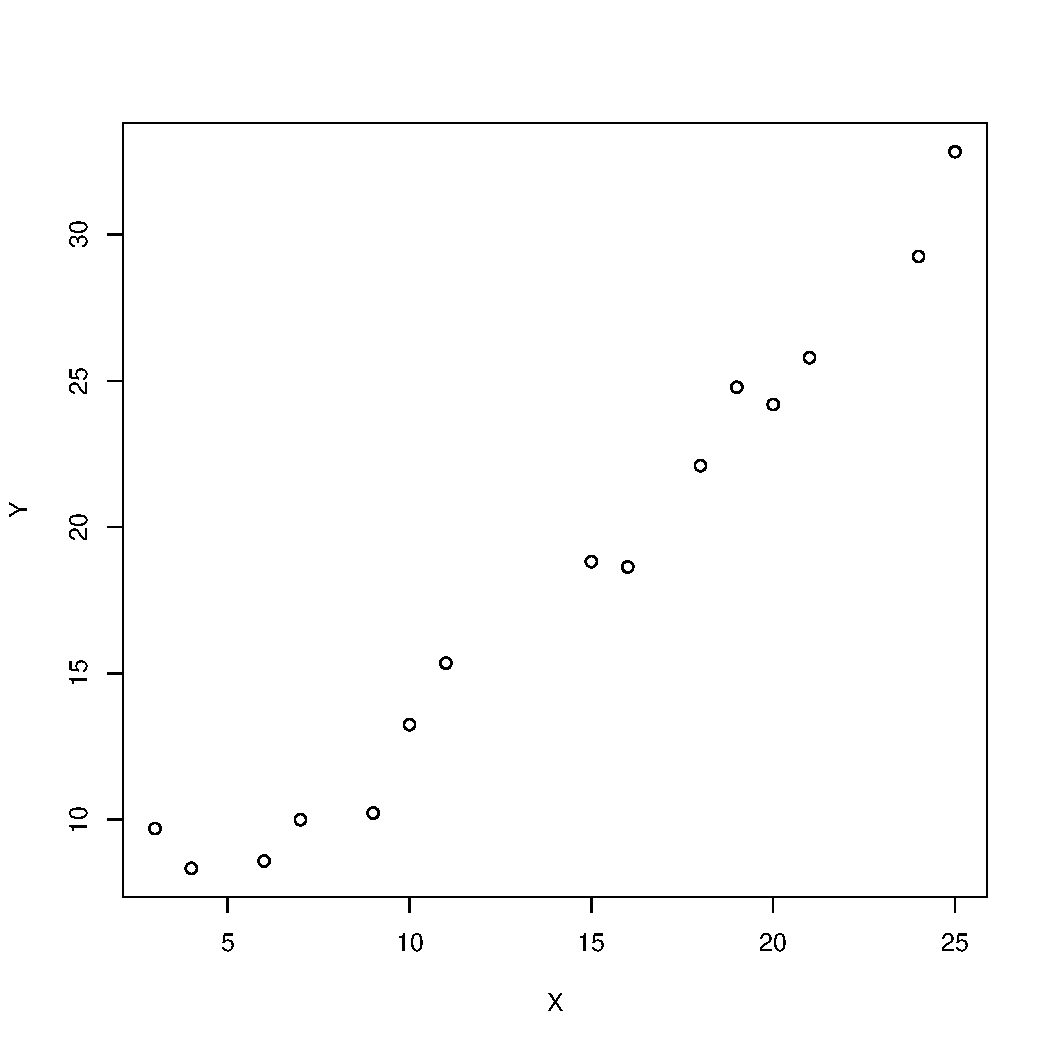
\includegraphics[width=\maxwidth]{figure/unnamed-chunk-52-1}

\end{knitrout}
      \caption{Graphique des données de l'exercice
        \ref{chap:multiple}.\ref{ex:multiple:quadratique}}
      \label{fig:multiple:quadratique}
    \end{figure}
    Par la suite, on peut estimer les paramètres de ce modèle avec la
    fonction \texttt{lm} de \textsf{R}:
\begin{knitrout}
\definecolor{shadecolor}{rgb}{0.969, 0.969, 0.969}\color{fgcolor}\begin{kframe}
\begin{alltt}
\hlstd{fit} \hlkwb{<-} \hlkwd{lm}\hlstd{(Y} \hlopt{~} \hlkwd{poly}\hlstd{(X,} \hlnum{2}\hlstd{),} \hlkwc{data} \hlstd{= donnees)}
\hlkwd{summary}\hlstd{(fit)}
\end{alltt}
\begin{verbatim}
##
## Call:
## lm(formula = Y ~ poly(X, 2), data = donnees)
##
## Residuals:
##     Min      1Q  Median      3Q     Max
## -1.9123 -0.6150 -0.1905  0.6367  1.6921
##
## Coefficients:
##             Estimate Std. Error t value Pr(>|t|)
## (Intercept)  18.1240     0.3025   59.91 3.10e-16 ***
## poly(X, 2)1  29.6754     1.1717   25.33 8.72e-12 ***
## poly(X, 2)2   4.0899     1.1717    3.49  0.00446 **
## ---
## Signif. codes:
## 0 '***' 0.001 '**' 0.01 '*' 0.05 '.' 0.1 ' ' 1
##
## Residual standard error: 1.172 on 12 degrees of freedom
## Multiple R-squared:  0.982,	Adjusted R-squared:  0.979
## F-statistic: 326.8 on 2 and 12 DF,  p-value: 3.434e-11
\end{verbatim}
\begin{alltt}
\hlkwd{anova}\hlstd{(fit)}
\end{alltt}
\begin{verbatim}
## Analysis of Variance Table
##
## Response: Y
##            Df Sum Sq Mean Sq F value    Pr(>F)
## poly(X, 2)  2 897.36  448.68  326.79 3.434e-11 ***
## Residuals  12  16.48    1.37
## ---
## Signif. codes:
## 0 '***' 0.001 '**' 0.01 '*' 0.05 '.' 0.1 ' ' 1
\end{verbatim}
\end{kframe}
\end{knitrout}
    Tant le test $F$ global que les tests $t$ individuels sont
    concluants, le coefficient de détermination est élevé et l'on peut
    constater à la figure \ref{fig:multiple:quadratique2} que
    l'ajustement du modèle est bon. On conclut donc qu'un modèle
    adéquat pour cet ensemble de données est
    \begin{displaymath}
      Y_t = 18,12 +
      29,68 X_t +
      4,09 X_t^2 + \varepsilon_t, \quad
      \varepsilon_t \sim N(0, 1,373).
    \end{displaymath}
    \begin{figure}
      \centering
\begin{knitrout}
\definecolor{shadecolor}{rgb}{0.969, 0.969, 0.969}\color{fgcolor}\begin{kframe}
\begin{alltt}
\hlkwd{plot}\hlstd{(Y} \hlopt{~} \hlstd{X,} \hlkwc{data} \hlstd{= donnees)}
\hlstd{x} \hlkwb{<-} \hlkwd{seq}\hlstd{(}\hlkwd{min}\hlstd{(donnees}\hlopt{$}\hlstd{X),} \hlkwd{max}\hlstd{(donnees}\hlopt{$}\hlstd{X),} \hlkwc{length} \hlstd{=} \hlnum{200}\hlstd{)}
\hlkwd{lines}\hlstd{(x,} \hlkwd{predict}\hlstd{(fit,} \hlkwd{data.frame}\hlstd{(}\hlkwc{X} \hlstd{= x),} \hlkwc{lwd} \hlstd{=} \hlnum{2}\hlstd{))}
\end{alltt}
\end{kframe}
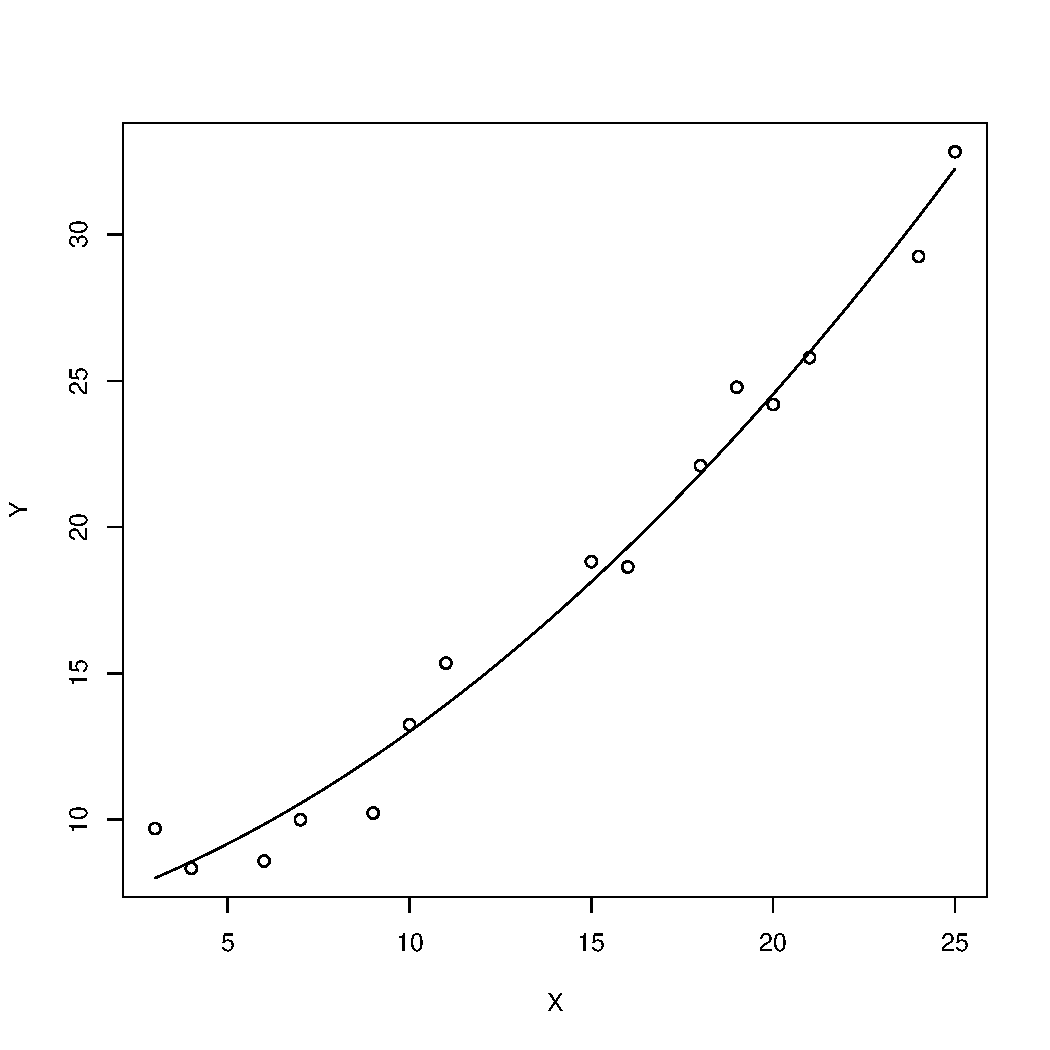
\includegraphics[width=\maxwidth]{figure/unnamed-chunk-54-1}

\end{knitrout}
      \caption{Graphique des données de l'exercice
        \ref{chap:multiple}.\ref{ex:multiple:quadratique} et courbe
        obtenue par régression}
      \label{fig:multiple:quadratique2}
    \end{figure}
  
\end{solution}
\begin{solution}{3.17}
    Comme on peut le constater à la figure \ref{fig:multiple:pondere},
    le point $(X_{16}, Y_{16})$ est plus éloigné des autres. En b) et
    c), on diminue son poids dans la régression.
    \begin{figure}
      \centering
\begin{knitrout}
\definecolor{shadecolor}{rgb}{0.969, 0.969, 0.969}\color{fgcolor}\begin{kframe}
\begin{alltt}
\hlkwd{plot}\hlstd{(Y} \hlopt{~} \hlstd{X,} \hlkwc{data} \hlstd{= donnees)}
\hlkwd{points}\hlstd{(donnees}\hlopt{$}\hlstd{X[}\hlnum{16}\hlstd{], donnees}\hlopt{$}\hlstd{Y[}\hlnum{16}\hlstd{],} \hlkwc{pch} \hlstd{=} \hlnum{16}\hlstd{)}
\end{alltt}
\end{kframe}
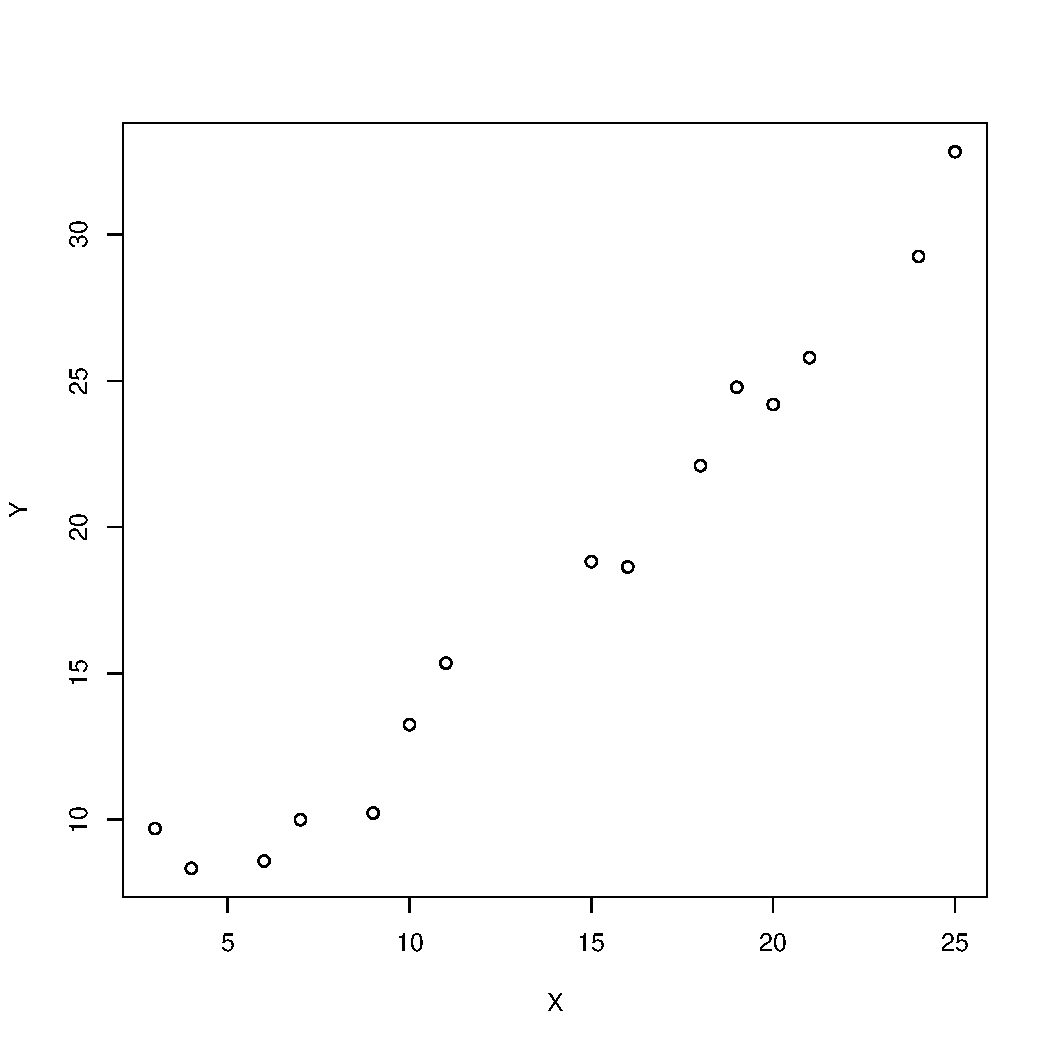
\includegraphics[width=\maxwidth]{figure/unnamed-chunk-56-1}

\end{knitrout}
      \caption{Graphique des données de l'exercice
        \ref{chap:multiple}.\ref{ex:multiple:pondere}. Le cercle plein
        représente la donnée $(X_{16}, Y_{16})$.}
      \label{fig:multiple:pondere}
    \end{figure}
    \begin{enumerate}
    \item On calcule d'abord l'estimateur des moindres carrés ordinaires:
\begin{knitrout}
\definecolor{shadecolor}{rgb}{0.969, 0.969, 0.969}\color{fgcolor}\begin{kframe}
\begin{alltt}
\hlstd{(fit1} \hlkwb{<-} \hlkwd{lm}\hlstd{(Y} \hlopt{~} \hlstd{X,} \hlkwc{data} \hlstd{= donnees))}
\end{alltt}
\begin{verbatim}
##
## Call:
## lm(formula = Y ~ X, data = donnees)
##
## Coefficients:
## (Intercept)            X
##      1.4256       0.3158
\end{verbatim}
\end{kframe}
\end{knitrout}
    \item Si l'on suppose que la variance de la données $(X_{16},
      Y_{16})$ est quatre fois plus élevée que la variance des autres
      données, alors il convient d'accorder un point quatre fois moins
      grand à cette donnée dans la régression. Cela requiert les
      moindres carrés pondérés. Pour calculer les estimateurs avec
      \texttt{lm} dans \textsf{R}, on utilise l'argument
      \texttt{weights}:
\begin{knitrout}
\definecolor{shadecolor}{rgb}{0.969, 0.969, 0.969}\color{fgcolor}\begin{kframe}
\begin{alltt}
\hlstd{w} \hlkwb{<-} \hlkwd{rep}\hlstd{(}\hlnum{1}\hlstd{,} \hlkwd{nrow}\hlstd{(donnees))}
\hlstd{w[}\hlnum{16}\hlstd{]} \hlkwb{<-} \hlnum{0.25}
\hlstd{(fit2} \hlkwb{<-} \hlkwd{update}\hlstd{(fit1,} \hlkwc{weights} \hlstd{= w))}
\end{alltt}
\begin{verbatim}
##
## Call:
## lm(formula = Y ~ X, data = donnees, weights = w)
##
## Coefficients:
## (Intercept)            X
##      1.7213       0.2243
\end{verbatim}
\end{kframe}
\end{knitrout}
    \item On répète la procédure en b) avec un poids de encore plus
      petit pour la donnée $(X_{16}, Y_{16})$:
\begin{knitrout}
\definecolor{shadecolor}{rgb}{0.969, 0.969, 0.969}\color{fgcolor}\begin{kframe}
\begin{alltt}
\hlstd{w[}\hlnum{16}\hlstd{]} \hlkwb{<-} \hlnum{0.0625}
\hlstd{(fit3} \hlkwb{<-} \hlkwd{update}\hlstd{(fit1,} \hlkwc{weights} \hlstd{= w))}
\end{alltt}
\begin{verbatim}
##
## Call:
## lm(formula = Y ~ X, data = donnees, weights = w)
##
## Coefficients:
## (Intercept)            X
##      1.8080       0.1975
\end{verbatim}
\end{kframe}
\end{knitrout}
      Plus le poids accordé à la donnée $(X_{16}, Y_{16})$ est faible,
      moins la droite de régression est attirée vers ce point (voir la
      figure \ref{fig:multiple:pondere2}).
      \begin{figure}[t]
        \centering
\begin{knitrout}
\definecolor{shadecolor}{rgb}{0.969, 0.969, 0.969}\color{fgcolor}\begin{kframe}
\begin{alltt}
\hlkwd{plot}\hlstd{(Y} \hlopt{~} \hlstd{X,} \hlkwc{data} \hlstd{= donnees)}
\hlkwd{points}\hlstd{(donnees}\hlopt{$}\hlstd{X[}\hlnum{16}\hlstd{], donnees}\hlopt{$}\hlstd{Y[}\hlnum{16}\hlstd{],} \hlkwc{pch} \hlstd{=} \hlnum{16}\hlstd{)}
\hlkwd{abline}\hlstd{(fit1,} \hlkwc{lwd} \hlstd{=} \hlnum{2}\hlstd{,} \hlkwc{lty} \hlstd{=} \hlnum{1}\hlstd{)}
\hlkwd{abline}\hlstd{(fit2,} \hlkwc{lwd} \hlstd{=} \hlnum{2}\hlstd{,} \hlkwc{lty} \hlstd{=} \hlnum{2}\hlstd{)}
\hlkwd{abline}\hlstd{(fit3,} \hlkwc{lwd} \hlstd{=} \hlnum{2}\hlstd{,} \hlkwc{lty} \hlstd{=} \hlnum{3}\hlstd{)}
\hlkwd{legend}\hlstd{(}\hlnum{1.2}\hlstd{,} \hlnum{6}\hlstd{,} \hlkwc{legend} \hlstd{=} \hlkwd{c}\hlstd{(}\hlstr{"Modèle a)"}\hlstd{,} \hlstr{"Modèle b)"}\hlstd{,} \hlstr{"Modèle c)"}\hlstd{),}
       \hlkwc{lwd} \hlstd{=} \hlnum{2}\hlstd{,} \hlkwc{lty} \hlstd{=} \hlnum{1}\hlopt{:}\hlnum{3}\hlstd{)}
\end{alltt}
\end{kframe}
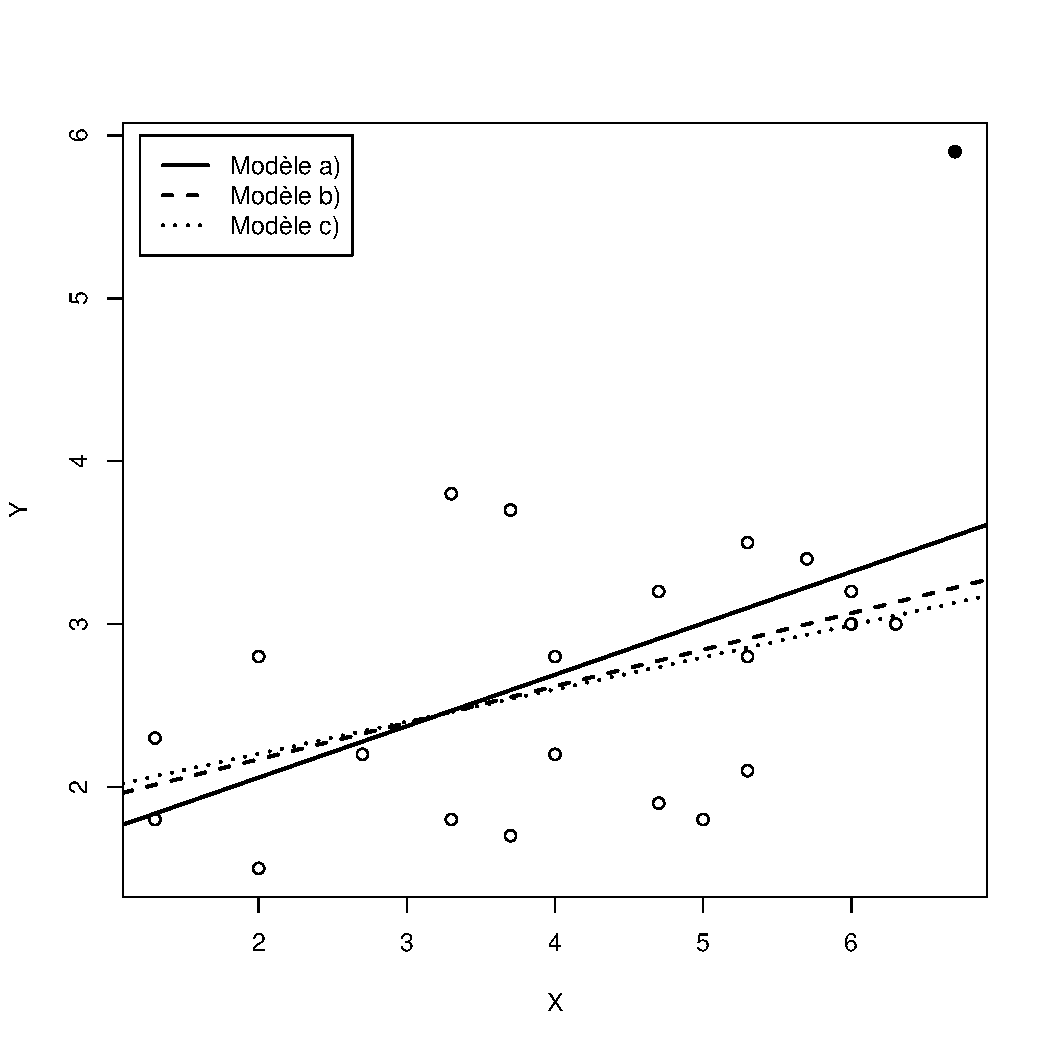
\includegraphics[width=\maxwidth]{figure/unnamed-chunk-60-1}

\end{knitrout}
        \caption{Graphique des données de l'exercice
          \ref{chap:multiple}.\ref{ex:multiple:pondere} avec les
          droites de régression obtenues à l'aide des moindres carrés
          pondérés.}
        \label{fig:multiple:pondere2}
      \end{figure}
    \end{enumerate}
  
\end{solution}
\begin{solution}{3.18}
    \begin{enumerate}
    \item Voir la figure \ref{fig:multiple:taxi} pour le graphique. Il
      y a effectivement une différence entre la consommation de
      carburant des hommes et des femmes: ces dernières font plus de
      milles avec un gallon d'essence.
      \begin{figure}
        \centering
\begin{knitrout}
\definecolor{shadecolor}{rgb}{0.969, 0.969, 0.969}\color{fgcolor}\begin{kframe}
\begin{alltt}
\hlstd{hommes} \hlkwb{<-} \hlkwd{subset}\hlstd{(donnees, sexe} \hlopt{==} \hlstr{"M"}\hlstd{)}
\hlstd{femmes} \hlkwb{<-} \hlkwd{subset}\hlstd{(donnees, sexe} \hlopt{==} \hlstr{"F"}\hlstd{)}
\hlkwd{plot}\hlstd{(mpg} \hlopt{~} \hlstd{age,} \hlkwc{data} \hlstd{= hommes,}
     \hlkwc{xlim} \hlstd{=} \hlkwd{range}\hlstd{(donnees}\hlopt{$}\hlstd{age),} \hlkwc{ylim} \hlstd{=} \hlkwd{range}\hlstd{(donnees}\hlopt{$}\hlstd{mpg))}
\hlkwd{points}\hlstd{(mpg} \hlopt{~} \hlstd{age,} \hlkwc{data} \hlstd{= femmes,} \hlkwc{pch} \hlstd{=} \hlnum{16}\hlstd{)}
\hlkwd{legend}\hlstd{(}\hlnum{4}\hlstd{,} \hlnum{16}\hlstd{,} \hlkwc{legend} \hlstd{=} \hlkwd{c}\hlstd{(}\hlstr{"Hommes"}\hlstd{,} \hlstr{"Femmes"}\hlstd{),} \hlkwc{pch} \hlstd{=} \hlkwd{c}\hlstd{(}\hlnum{1}\hlstd{,} \hlnum{16}\hlstd{))}
\end{alltt}
\end{kframe}
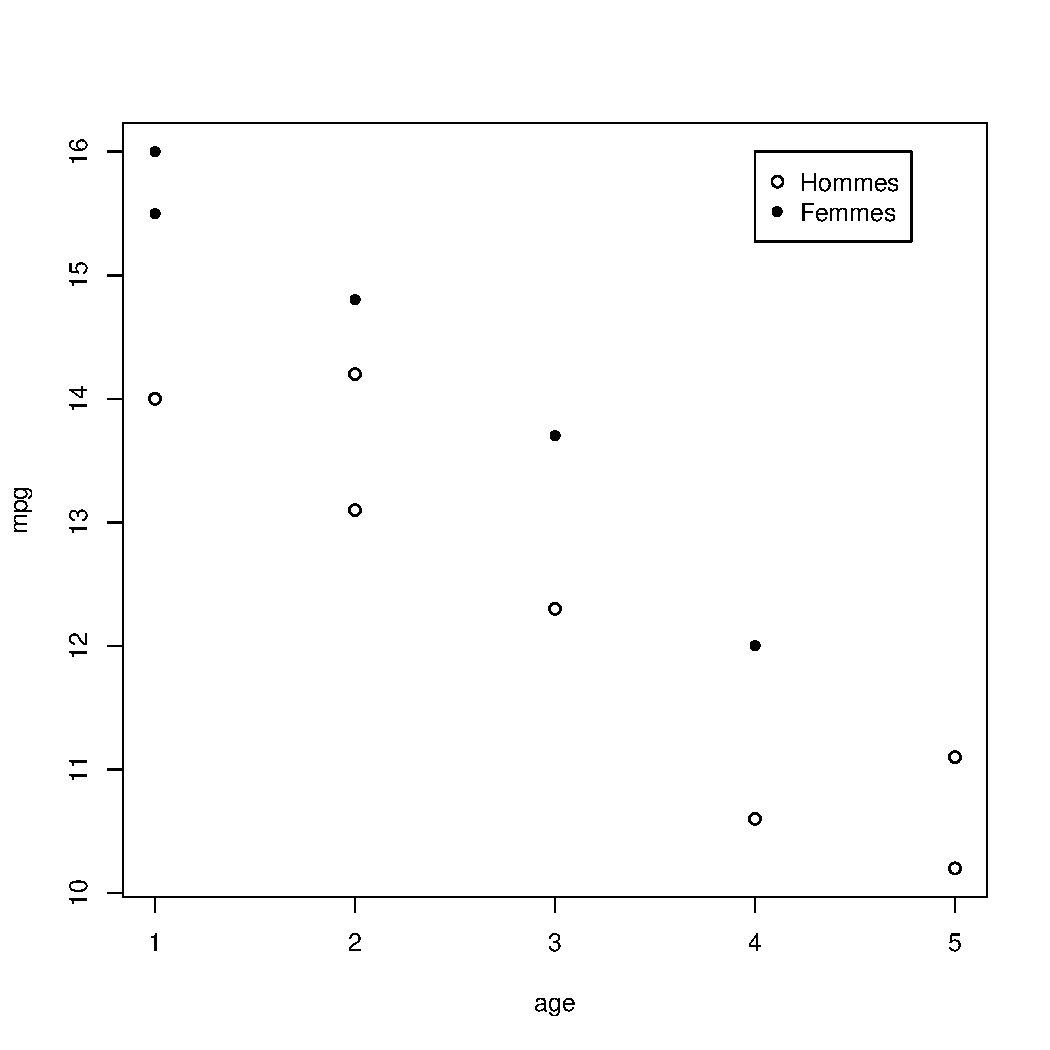
\includegraphics[width=\maxwidth]{figure/unnamed-chunk-62-1}

\end{knitrout}
        \caption{Graphique des données de l'exercice
          \ref{chap:multiple}.\ref{ex:multiple:taxi}}
        \label{fig:multiple:taxi}
      \end{figure}
    \item Remarquer que la variable \texttt{sexe} est un facteur et peut
      être utilisée telle quelle dans \texttt{lm}:
\begin{knitrout}
\definecolor{shadecolor}{rgb}{0.969, 0.969, 0.969}\color{fgcolor}\begin{kframe}
\begin{alltt}
\hlstd{(fit} \hlkwb{<-} \hlkwd{lm}\hlstd{(mpg} \hlopt{~} \hlstd{age} \hlopt{+} \hlstd{sexe,} \hlkwc{data} \hlstd{= donnees))}
\end{alltt}
\begin{verbatim}
##
## Call:
## lm(formula = mpg ~ age + sexe, data = donnees)
##
## Coefficients:
## (Intercept)          age        sexeM
##      16.687       -1.040       -1.206
\end{verbatim}
\end{kframe}
\end{knitrout}
    \item Calcul d'une prévision pour la valeur moyenne de la variable
      \texttt{mpg}:
\begin{knitrout}
\definecolor{shadecolor}{rgb}{0.969, 0.969, 0.969}\color{fgcolor}\begin{kframe}
\begin{alltt}
\hlkwd{predict}\hlstd{(fit,} \hlkwc{newdata} \hlstd{=} \hlkwd{data.frame}\hlstd{(}\hlkwc{age} \hlstd{=} \hlnum{4}\hlstd{,} \hlkwc{sexe} \hlstd{=} \hlstr{"F"}\hlstd{),}
        \hlkwc{interval} \hlstd{=} \hlstr{"confidence"}\hlstd{,} \hlkwc{level} \hlstd{=} \hlnum{0.90}\hlstd{)}
\end{alltt}
\begin{verbatim}
##        fit      lwr      upr
## 1 12.52876 11.94584 13.11168
\end{verbatim}
\end{kframe}
\end{knitrout}
    \end{enumerate}
  
\end{solution}
\begin{solution}{3.19}
\begin{enumerate}
\item Le postulat de normalité semble violé.

La distribution des résidus a une queue inférieure plus épaisse que la loi normale, ce que l'on voit à gauche du Q-Q plot, puisque les poits ne sont pas alignés.

Le postulat de normalité n'est pas critique, parce que les estimateurs des moindres carrés ont un sens quand même. Toutefois, les tests d'hypothèses et les intervalles de confiance ne sont pas valides.

\item Le graphique des résidus en fonction de $x_2$ montre que le postulat de linéarité semble violé. Cela implique que le modèle n'est pas valide.

On observe de l'hétéroscédasticité (par exemple, dans les graphiques 1, 3 ou 4) puisque les résidus ne semblent pas avoir une variance constante.

Cela signifie que les variances des paramètres ne sont pas calculées de façon appropriée OU il faudrait effectuer une transformation sur les variables pour régler ces problèmes.


\end{enumerate}
\end{solution}
\begin{solution}{3.20}
On pourrait croire qu'un point sur 20, ça ne change rien, mais ce n'est pas le cas! Le point 1 a un impact sur la pente et la qualité de l'ajustement. Le point 2 a un grand levier mais n'affecte pas beaucoup les estimations, le point 3 a un grand levier et un gros impact.

\begin{verbatim}
dat <- read.csv("OutlierExample.csv")

dim(dat)

summary(dat)

library(ggplot2)

ggplot(dat, aes(x= X, y= Y, label=CODES))+
  geom_point() +
  geom_text(aes(label=ifelse(CODES>0,CODES,'')),hjust=0,vjust=0)

fit0 <- lm(Y~X,dat,subset=(CODES==0))
summary(fit0)
plot(dat[,1:2],pch=16)
points(dat[match(1:3,dat$CODES),1:2],col=2:4,pch=16:18,cex=1.2)
abline(fit0)

fit1 <- lm(Y~X,dat,subset=(CODES<=1))
summary(fit1)
abline(fit1,col=2,lty=2)

fit2 <- lm(Y~X,dat,subset=(CODES%in%c(0,2)))
summary(fit2)
abline(fit2,col=3,lty=3)

fit3 <- lm(Y~X,dat,subset=(CODES%in%c(0,3)))
summary(fit3)
abline(fit3,col=4,lty=4)

influence.measures(fit0)
influence.measures(fit1)
influence.measures(fit2)
influence.measures(fit3)

\end{verbatim}
\end{solution}
